\begin{figure}[htbp]
\centering
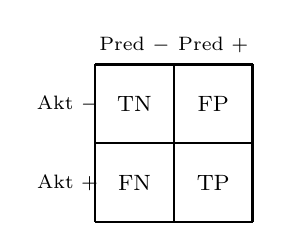
\begin{tikzpicture}[scale=1.0]
  \draw[thick] (0,0) grid (2,2);
  \node at (0.5,1.5) {\footnotesize TN};
  \node at (1.5,1.5) {\footnotesize FP};
  \node at (0.5,0.5) {\footnotesize FN};
  \node at (1.5,0.5) {\footnotesize TP};
  \node[font=\scriptsize] at (0.5,2.25) {Pred $-$};
  \node[font=\scriptsize] at (1.5,2.25) {Pred $+$};
  \node[font=\scriptsize] at (-0.35,1.5) {Akt $-$};
  \node[font=\scriptsize] at (-0.35,0.5) {Akt $+$};
\end{tikzpicture}
\caption{Sketsa confusion matrix biner: TP/TN benar; FP/FN salah. Presisi dan recall membobot jenis kesalahan secara berbeda.}
\end{figure}
